\subsubsection{Bellman-Ford (Caminho Mínimo com Pesos Negativos)}
O algoritmo de Bellman-Ford é utilizado para encontrar caminhos mínimos em
grafos que contêm arestas com pesos negativos. Ao contrário do Dijkstra, ele
relaxa todas as arestas do grafo repetidas vezes ($V-1$ vezes, onde $V$ é o
número de vértices). Se no $V$-ésimo passo ainda for possível relaxar alguma
aresta, significa que existe um \textbf{ciclo de peso negativo} no grafo. Sua complexidade é: $\mathcal{O}(V * E)$

\paragraph{Pseudo-Código: }\mbox{}\\
\begin{algorithm}[H]
	\SetAlgoLined
	\SetKwFunction{BellmanFord}{BellmanFord}
	\SetKwProg{Fn}{Função}{:}{}

	\Fn{\BellmanFord{$inicio, arestas, V$}}{
		$dist \gets$ array de tamanho $V$ inicializado com $\infty$\;
		$dist[inicio] \gets 0$\;

		\Para{$i \gets 1$ \Ate $V - 1$}{
			\ParaCada{$(u, v, peso) \in arestas$}{
				\Se{$dist[u] + peso < dist[v]$}{
					$dist[v] \gets dist[u] + peso$\;
				}
			}
		}

		\ParaCada{$(u, v, peso) \in arestas$}{
			\Se{$dist[u] + peso < dist[v]$}{
				\Retorna \text{Ciclo negativo detectado}\;
			}
		}
	}
	\caption{Algoritmo de BellmanFord}
\end{algorithm}

Veja uma iteração de relaxamento do Bellman-Ford:\\ \vspace{0.5cm} \noindent
\begin{minipage}[t]{0.31\textwidth}
	\centering
	\textbf{Passo 1: Estado Inicial}\\
	\vspace{0.2cm}
	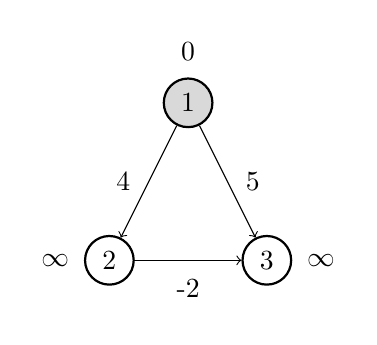
\begin{tikzpicture}[every node/.style={circle, draw, minimum size=0.5cm, thick}]
		\node[fill=gray!30, label=above:{$0$}] (1) at (0, 1) {1};
		\node[label=left:{$\infty$}] (2) at (-1, -1) {2};
		\node[label=right:{$\infty$}] (3) at (1, -1) {3};
		\draw[->] (1) -- node[left, draw=none, fill=none] {4} (2);
		\draw[->] (1) -- node[right, draw=none, fill=none] {5} (3);
		\draw[->] (2) -- node[below, draw=none, fill=none] {-2} (3);
	\end{tikzpicture}

	\vspace{0.2cm}
	\footnotesize
	\raggedright
	Distâncias iniciais: $dist[1]=0$, outros $\infty$.
\end{minipage}%
\hfill
%
\begin{minipage}[t]{0.31\textwidth}
	\centering
	\textbf{Passo 2: Relaxando 1 $\to$ 2 e 1 $\to$ 3}\\
	\vspace{0.2cm}
	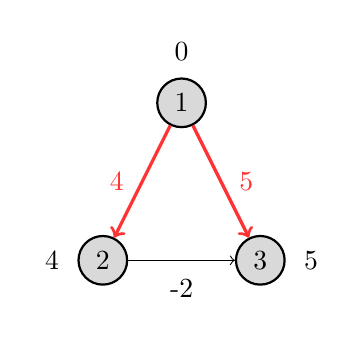
\begin{tikzpicture}[every node/.style={circle, draw, minimum size=0.5cm, thick}]
		\node[fill=gray!30, label=above:{$0$}] (1) at (0, 1) {1};
		\node[fill=gray!30, label=left:{$4$}] (2) at (-1, -1) {2};
		\node[fill=gray!30, label=right:{$5$}] (3) at (1, -1) {3};
		\draw[->, very thick, red!80] (1) -- node[left, draw=none, fill=none] {4} (2);
		\draw[->, very thick, red!80] (1) -- node[right, draw=none, fill=none] {5} (3);
		\draw[->] (2) -- node[below, draw=none, fill=none] {-2} (3);
	\end{tikzpicture}

	\vspace{0.2cm}
	\footnotesize
	\raggedright
	$dist[2] = 4$, $dist[3] = 5$.
\end{minipage}%
\hfill
%
\begin{minipage}[t]{0.31\textwidth}
	\centering
	\textbf{Passo 3: Relaxando 2 $\to$ 3}\\
	\vspace{0.2cm}
	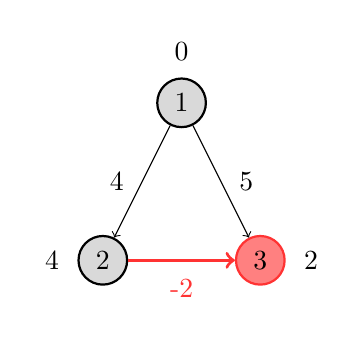
\begin{tikzpicture}[every node/.style={circle, draw, minimum size=0.5cm, thick}]
		\node[fill=gray!30, label=above:{$0$}] (1) at (0, 1) {1};
		\node[fill=gray!30, label=left:{$4$}] (2) at (-1, -1) {2};
		\node[fill=red!50, draw=red!80, label=right:{$2$}] (3) at (1, -1) {3};
		\draw[->] (1) -- node[left, draw=none, fill=none] {4} (2);
		\draw[->] (1) -- node[right, draw=none, fill=none] {5} (3);
		\draw[->, very thick, red!80] (2) -- node[below, draw=none, fill=none] {-2} (3);
	\end{tikzpicture}

	\vspace{0.2cm}
	\footnotesize
	\raggedright
	$dist[2] + (-2) < dist[3]$. Logo $dist[3] = 2$.
\end{minipage}

\paragraph{Implementação: }\mbox{}\\
\textbf{Python: }
\begin{lstlisting}[language=Python]
def bellman_ford(inicio, n, arestas):
    dist = [float('inf')] * n
    dist[inicio] = 0
    
    for _ in range(n - 1):
        for u, v, peso in arestas:
            if dist[u] != float('inf') and dist[u] + peso < dist[v]:
                dist[v] = dist[u] + peso
                
    # Verificacao de ciclo negativo
    for u, v, peso in arestas:
        if dist[u] != float('inf') and dist[u] + peso < dist[v]:
            return None 
            
    return dist
\end{lstlisting}

\vspace{0.3cm}
\textbf{C++:}
\begin{lstlisting}[language=C++]
struct Aresta {
    int u, v, peso;
};

vector<int> bellman_ford(int inicio, int n, const vector<Aresta>& arestas) {
    vector<int> dist(n, 1e9);
    dist[inicio] = 0;
    
    for (int i = 0; i < n - 1; ++i) {
        for (const auto& a : arestas) {
            if (dist[a.u] < 1e9 && dist[a.u] + a.peso < dist[a.v]) {
                dist[a.v] = dist[a.u] + a.peso;
            }
        }
    }
    
    for (const auto& a : arestas) {
        if (dist[a.u] < 1e9 && dist[a.u] + a.peso < dist[a.v]) {
            return {}; // Retorna vetor vazio se houver ciclo negativo
        }
    }
    return dist;
}
\end{lstlisting}
\newpage